\documentclass[fullpage,11pt]{article}
\usepackage[a4paper,left=2cm,top=2cm,right=2cm,bottom=2.5cm]{geometry}
\usepackage{amsfonts,amsmath,amsthm,array,amssymb}
\usepackage{hyperref}
%\usepackage[sort&compress]{natbib}
\usepackage{cite}
\usepackage{indentfirst}
\usepackage{color}
\usepackage{fullpage}
\renewcommand{\familydefault}{\sfdefault}
\usepackage{xcolor}
\usepackage{graphicx,wrapfig}
\usepackage[font={small}]{caption}
\pagenumbering{gobble}

\begin{document}  

\noindent Dear Editor,

\noindent We are submitting a Presubmission Inquiry for a Software article describing our open source library Microvessel Chaste.  We now overview how we believe the software and article meet the requirements of the journal.

\subsubsection*{Outstanding open source software of exceptional importance}
The Microvessel Chaste library is for composing multi-scale agent-based models of tissues with microvessels. Models of this type are used by many research groups and have broad and important applications in studying vascularized tumours [1-3], angiogenesis and vascular patterning [4, 5, 6],  osteogenesis [7] and oxygen transport [8]. While there are many bespoke computational models for these applications, there is not yet a general open source software framework for easily composing them (in the same way that Chaste or CompuCell3D can be used for agent-based cell models). The value of such a framework has been independently recognized in the literature [9], and feasibility has been previously demonstrated by others [6].

The design of Microvessel Chaste focuses on easy and reliable composition of computationally efficient models of vascularized tissues. Extensibility and efficiency are gained through object-oriented programming in C++, reliability through automated dimensional analysis and unit-testing, and user-friendliness through API documentation, web-based tutorials and a Python interface. An overview of code design and a brief literature review of vascularized tissue models will be included in the first two sections of the article.

\subsubsection*{New biological insights}
The Microvessel Chaste library is based on computational models and software built over a period of a decade by the authors, which are being made available open source for the first time. These models have previously been used to gain biological insights in the areas of tumour radiotherapy [10], tumour growth [11] and chemo- and anti-angiogenic therapy design [12, 13]. The library has been developed in close collaboration with experimentalist colleagues at the CRUK/MRC Institute for Radiation Oncology, University of Oxford and is focused on integration of experimental measurements (particularly imaging data of the type in Fig. 1 (a)) with modelling. An application of the library with multi-photon imaging data in the study of tumour radiotherapy is described in Grogan et al.~[10].

The article will link to a web-based ‘Paper Tutorial’ with two fully reproducible sample problems of biological interest, a 2D lattice-based tumour growth model to demonstrate replication of a common model in the literature [13] (see Fig. 1 for an example output) and a 3D off-lattice angiogenesis model corresponding to the corneal micro-pocket experimental assay [14] (see Fig. 2 for an example experiment and model output). The latter introduces advanced features of the library including off-lattice angiogenesis and PDE solution in complex 3D geometries (for example, hemispherical shells). Modification of these example problems should allow the reader to study a range of problems of biological interest.

\begin{figure}[!h]
\centering
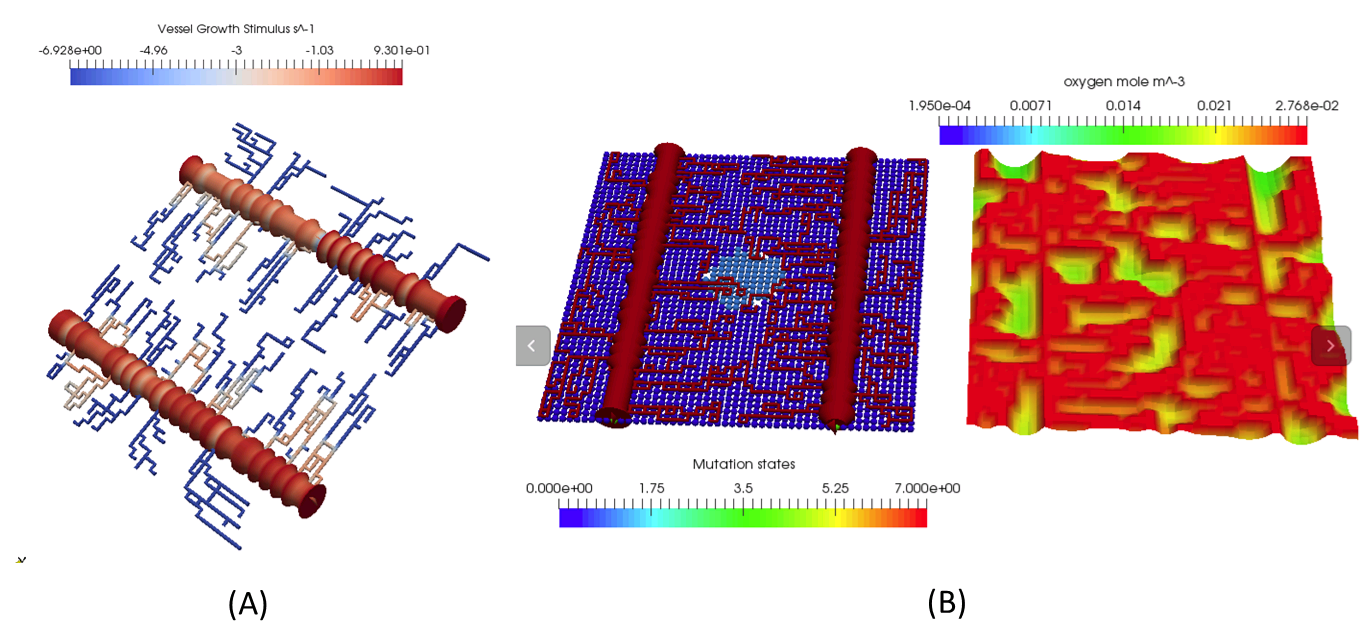
\includegraphics[width=0.65\textwidth]{Fig3.png}
\caption{{\bf A 2D lattice-based tumour simulation performed using the Microvessel Chaste library.}
(a) An experimental image of a tumour microvessel network (red) following administration of a Hoescht stain (blue), which stains DNA in cells [10]. (b) A computational model of tumour growth over a period of 16 days using the Microvessel Chaste library, including angiogenesis, blood-flow driven structural adaptation, oxygen and VEGF transport and cell-cycling.}
\label{fig3}
\end{figure}

\begin{figure}[!h]
\centering
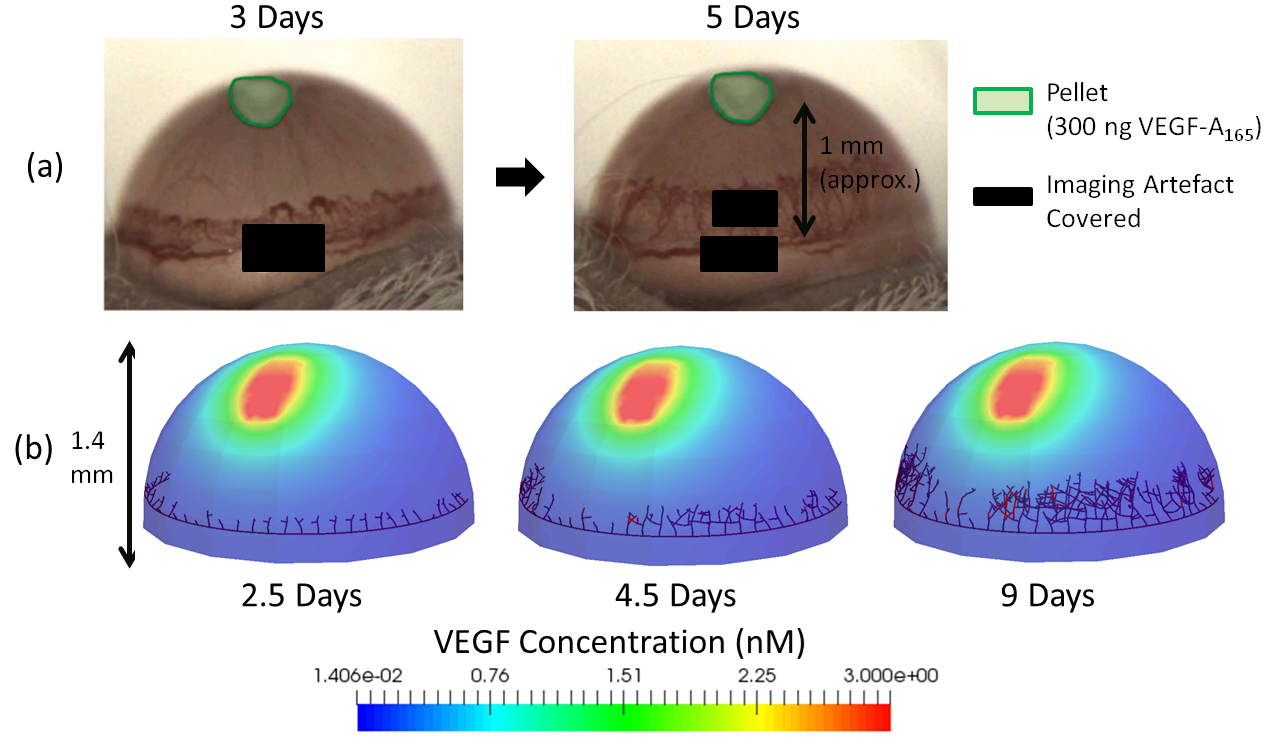
\includegraphics[width=0.75\textwidth]{Fig4.png}
\caption{{\bf A 3D off-lattice angiogenesis simulation performed using the Microvessel Chaste library.}
(a) Images from a cornea micropocket experiment showing microvessels (dark red) at 3-5 days post pellet implantation [14]. (b) Application of the Microvessel Chaste library in modelling a similar experiment.}
\label{fig4}
\end{figure}

\subsubsection*{Widely adopted or promise of wide adoption by broad community}
The article will compliment the first public release of the Microvessel Chaste library. However, we believe that there is potential for wide adoption in future. The library can be used as a plug-in for the Cell-Based Chaste software [15] (adding significant new functionality), without any additional dependencies. Cell-Based Chaste has been widely used in soft tissue modelling [15] and it is envisaged that the Microvessel Chaste library will be of interest to many of its users. The availability of a Python interface, detailed documentation and the use of common build (CMake), version control (git/Github) and input and output formats (VTK) will further help adoption. Development of the software is active for the foreseeable future, as it is the focus of on-going research on integration of multi-photon imaging and multi-scale modelling of tumour growth.

\subsubsection*{Downloadable anonymously in source code form}
The library is available under a permissive open source license (BSD 3-clause) on Github (\url{https://jmsgrogan.github.io/MicrovesselChaste/}) and can be built from source using standard tools. A dedicated Github account is available for anonymous code download and documentation access by reviewers. The repository will be made public following review.

In summary, we propose a Software article describing our new library, Microvessel Chaste. We believe the library will ease the composition of 2D and 3D multi-scale agent-based models of vascularized tissue and will be useful for other researchers in a broad range of applications in biology. The article will: i) overview the literature on multi-scale agent-based modelling of vascularized tissue, ii) overview the main features of the code through a flow-chart based demonstration of model composition and solution, iii) demonstrate a 2D lattice-based tumour growth problem, iv) demonstrate a 3D off-lattice angiogenesis problem and v) describe how the code can be obtained.

\noindent We look forward to your response, \\ James Grogan (on behalf of the authors)\\

\noindent Authors: 

James Grogan, Anthony Connor, Philip Maini, Helen Byrne and Joe Pitt-Francis, Mathematical Institute and Dept. of Computer Science, University of Oxford.

Bostjan Markelc and Ruth Muschel, CRUK/MRC Institute for Radiation Oncology, University of Oxford.

\subsubsection*{References}

[1] Frieboes HB, Lowengrub JS, Wise S, Zheng X, Macklin P, Bearer E, Cristini V. Computer simulation of glioma growth and morphology. Neuroimage. 2007;37(Supl 1):S59-S70.

[2] Shirinifard A, Scott Gens J, Zaitlen L, Poplawski J, Swat M, Glazier JA. 3D multi-cell simulation of tumor growth and angiogenesis. PLoS One. 2009;4(10):e7190.

[3] Welter M, Rieger H. Interstitial fluid flow and drug delivery in vascularized tumors: a computational model. PLoS One. 2013;8(8):e70395.

[4] Secomb TW, Alberding JP, Hsu R, DeWhirst MW, Pries AR. Angiogenesis: an adaptive dynamic biological patterning problem. PLoS Comput Biol. 2013;9(3):e1002983.

[5] Boas SEM, Merks RMH. Tip cell overtaking occurs as a side effect of sprouting in computational models of angiogenesis. BMC Systems Bio. 2015;9(86):DOI 10.1186/s12918-015-0230-7.

[6] Liu G, Qutub AA, Vempati P, Mac Gabhann F, Popel AS. Module-based multiscale simulation of angiogenesis in skeletal muscle. Theor Biol Med Model. 2011;8(6):DOI: 10.1186/1742-4682-8-6.

[7] Carlier A, Geris L, Bentley K, Carmeliet G, Carmeliet P, Van Oosterwyck H. MOSAIC: A multiscale model of osteogenesis and sprouting angiogenesis with lateral inhibition of endothelial cells. PLoS Comput Biol. 2012;8(10):e1002724.

[8] Beard DA, Bassingthwaighte JB. Modeling advection and diffusion of oxygen in complex vascular
networks. Ann Biomed Eng. 2001;29:298-310.

[9] Rieger H, Welter M. Integrative models of vascular remodeling during tumor growth. WIREs Syst Biol Med. 2015;7:113-129.

[10] Grogan JA, Markelc B, Connor AJ, Muschel R, Pitt-Francis JM, Maini PK, Byrne HM. Predicting the influence of microvascular structure on tumour response to radiotherapy. IEEE Trans Biomed Eng. 2016;DOI:10.1109/TBME.2016.2606563.

[11] Perfahl H, Byrne HM, Chen T, Estrella V, Alarcon T, Lapin A, Gatenby R, Gillies RJ, Llord MC, Maini PK, Reuss M, Owen MR. Multiscale modelling of vascular tumour growth in 3D: the roles of domain size and boundary conditions. PLoS One. 2011 April;6(4):e14790.

[12] Alarcon T, Owen MR, Byrne HM, Maini PK. M ultiscale modelling of tumour growth and therapy: the influence of vessel normalisation on chemotherapy. Computat and Math Method in Med. 2006;7(2-3):85-119.

[13] Owen MR, Stamper J, Muthana M, Richardshon GW, Dobson J, Lewis CE, Byrne HM. Mathematical modeling predicts synergistic antitumor effects of combining a macrophage-based, hypoxia-targeted gene therapy with chemotherapy. Cancer Res. 2015 April;71(8):2826-2837.

[14] Connor AJ, Radoslaw P, Nowak EL, Thomas M, Hertig F, Hoert S, Quaiser T, Schocat E, Pitt-Francis J, Cooper J, Maini PK, Byrne HM. An integrated approach to quantitative modelling in angiogenesis research. J R Soc Interface. 2015 August;12:e20150546.

[15] Mirams GR, Arthurs CJ, Bernabeu MO, Bordas R, Cooper J, Corrias A, Davit Y, Dunn S, Fletcher AG, Harvey DG, Marsh ME, Osborne JM, Pathmanathan P, Pitt-Francis J, Southern J, Zemzemi N, Gavaghan DJ. Chaste: an open source C++ library for computational physiology and biology. PLoS Comput Biol. 2013 Jan;9(3):e1002970.

\end{document}













